%%%%%%%%%%%%%%%%%%%%%%%%%%%%%%%%%%%%%%%%%%%%%%
%                insertmeeting
% 1) Title (something creative & funny?)
% 2) Date (MM/DD/YYYY)
% 3) Location (ex. Hagerty High School)
% 4) People/Committees Present 
% 5) Picture 
% 6) Start Time & Stop Time (ex. 12:30AM to 4:30PM)
%%%%%%%%%%%%%%%%%%%%%%%%%%%%%%%%%%%%%%%%%%%%%%
\insertmeeting 
	{ARMaggedon} 
	{11/05/21}
	{Hagerty High School}
	{Annika, Clayton, Nathan, Ritam}
	{Images/RobotPics/robot.jpg}
	{2:30 - 4:30}
	
\hhscommittee{Hardware}
\noindent\hfil\rule{\textwidth}{.4pt}\hfil
\subsubsection*{Goals}
\begin{itemize}
    \item Make arm reach higher
    \item Test with driver practice  

\end{itemize} 

\noindent\hfil\rule{\textwidth}{.4pt}\hfil

\subsubsection*{Accomplishments}
Following our exciting scrimmage with 4227 yesterday, we were left with very clear objectives of what needed to be fixed on the robot. The main thing we want to focus on today is the height of the arm. We found during the scrimmage that the arm wasn’t long enough to reach to the top of the alliance shipping hub when it was tilted away from us. Although we could simply make the rev extrusion we use as the arm longer, this would make it harder for our robot to fit within the 18 inch size requirements. Instead, we came up with the idea of moving the arm’s pivot point upwards to give it an extra 1.5 inches of reach, just enough to reach the highest level when tilted. To do this we had to replace the structure holding up the arm and motor with longer rev extrusions so we could shift everything up (Figure \ref{fig:pic1})


\begin{figure}[htp]
\centering
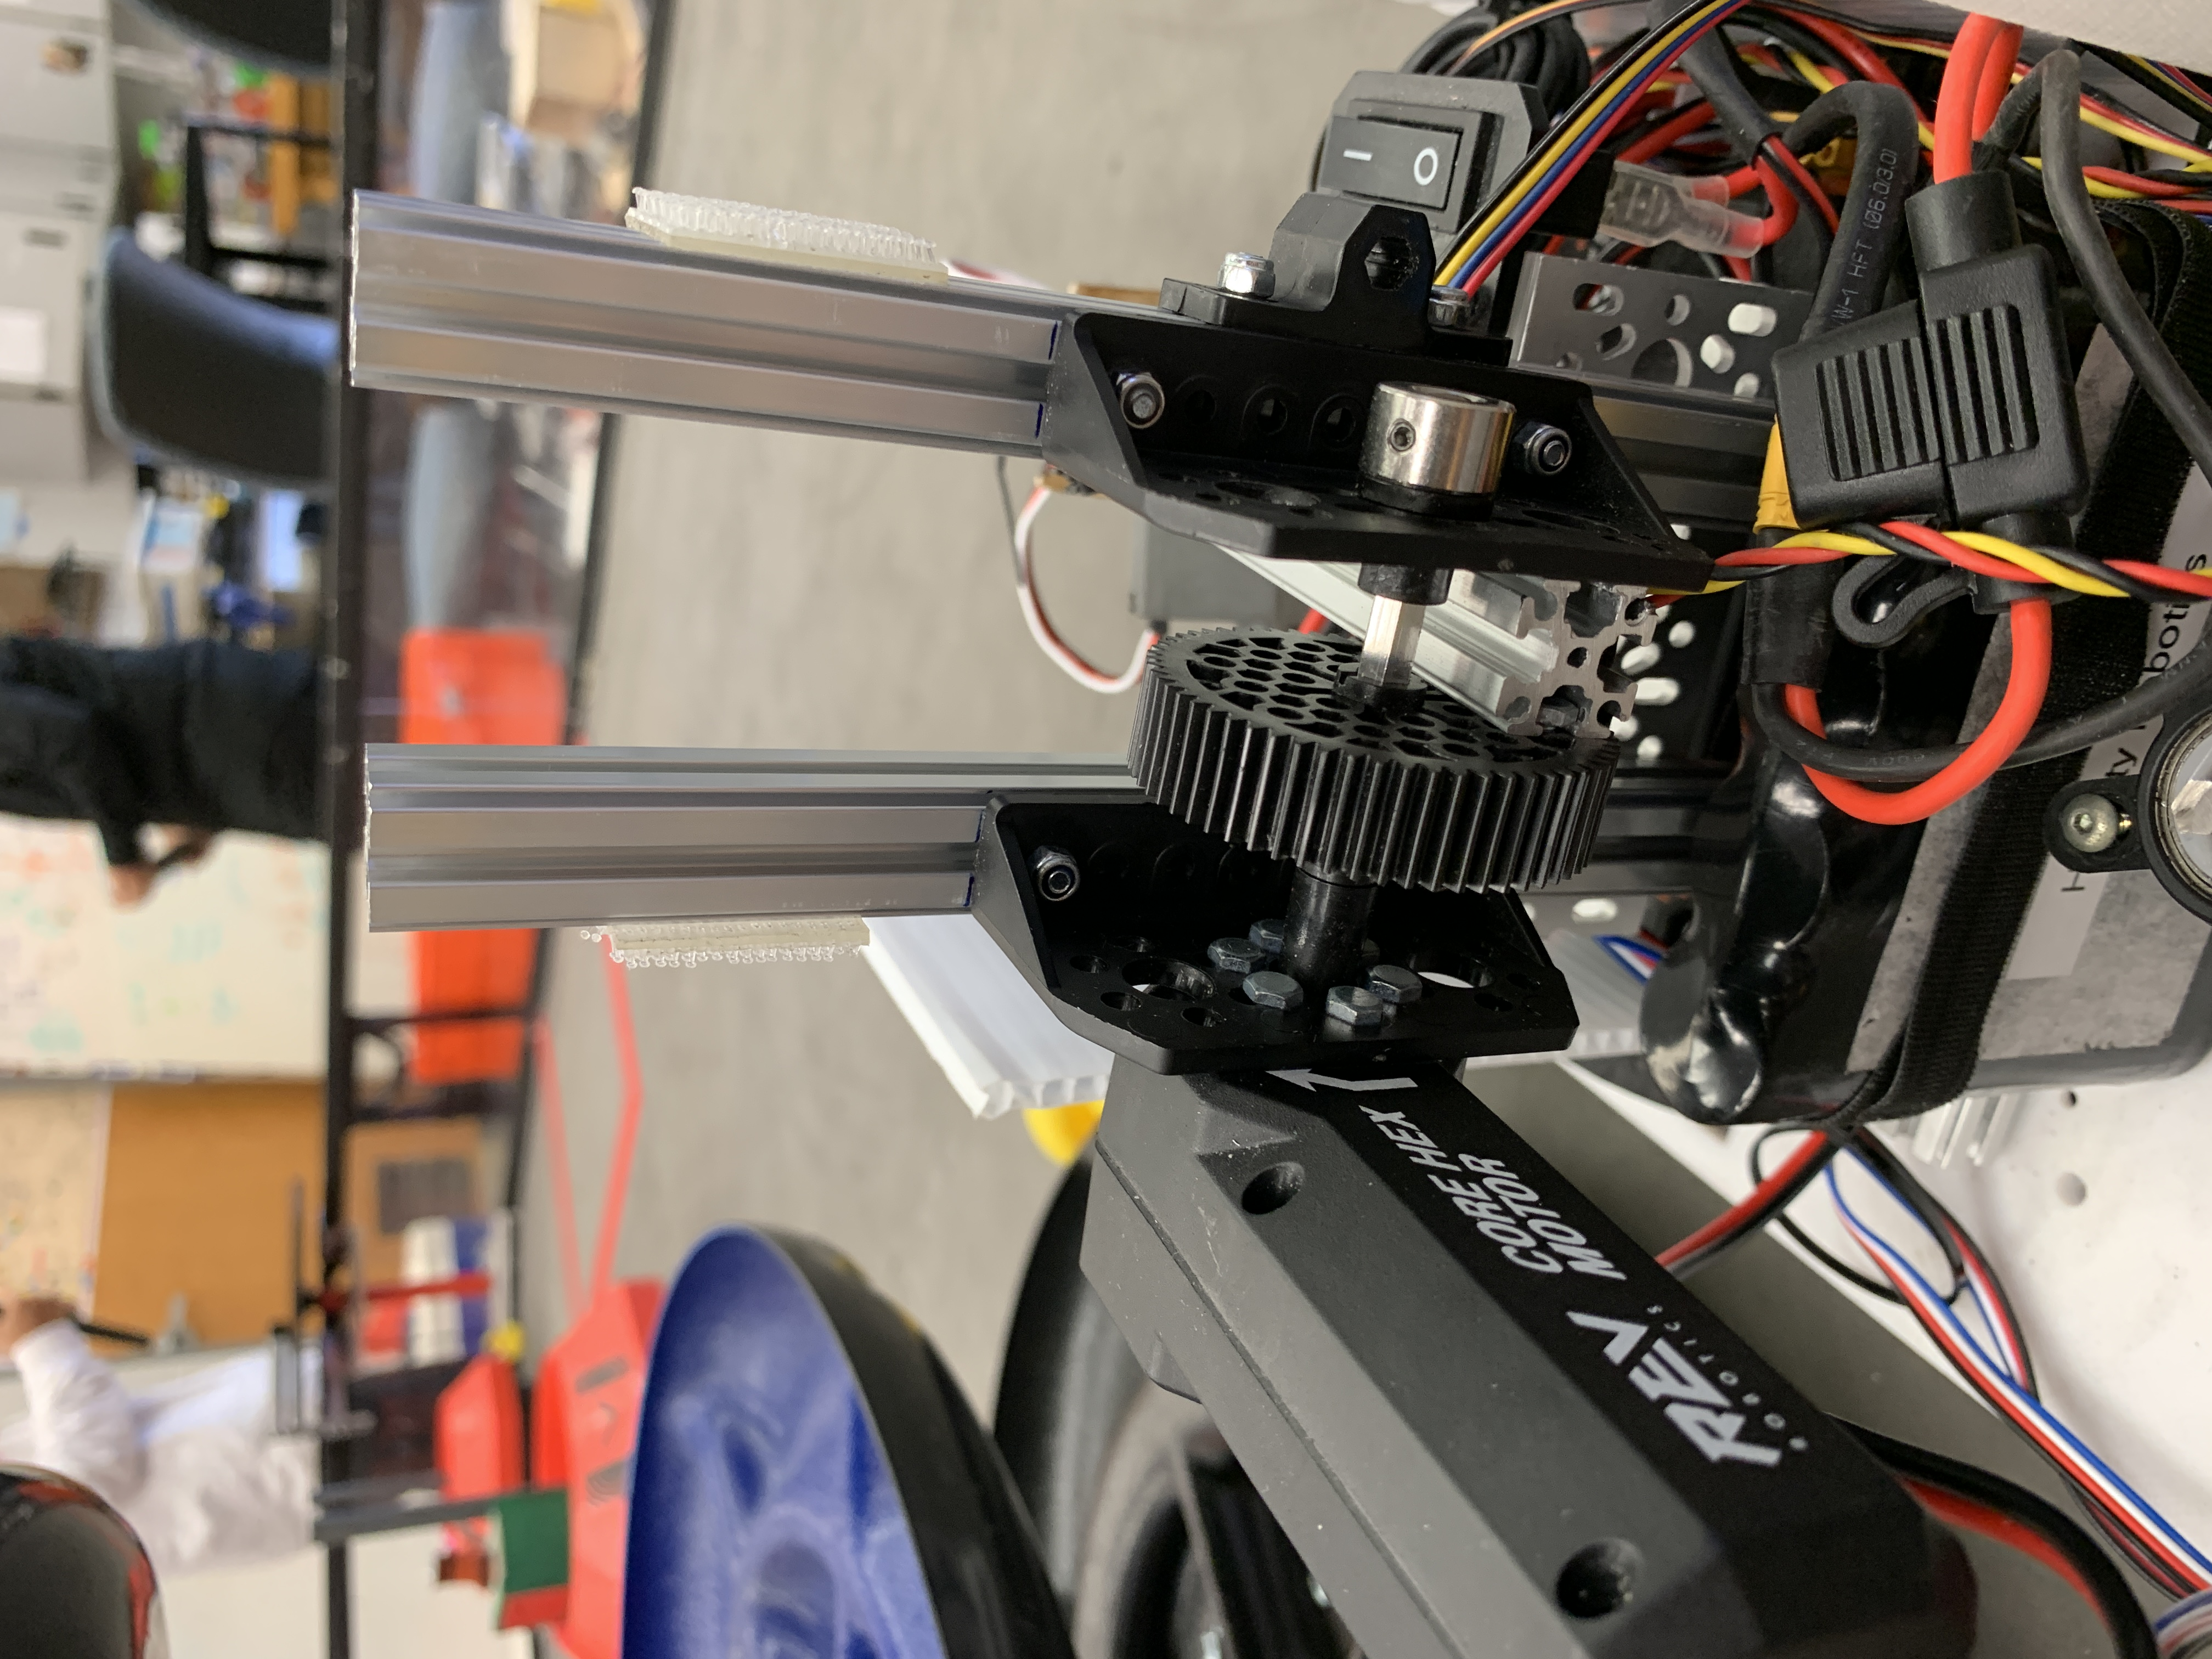
\includegraphics[width=0.95\textwidth, angle=0]{Meetings/November/11-05-21/11-5-21_Hardware_Figure 1 - Nathan Forrer.JPG}
\caption{The arm with new extrusions}
\label{fig:pic1}
\end{figure}

\whatsnext{
\begin{itemize}
    \item Add numbers onto robot
    \item Make sure robot fits in 18 inches
\end{itemize} 
}

